\section{Rover}

%TODO List the following infos about the rover:
%Software
%Communication protocols
%Sensors/actuators
%Users and user stories


\subsection{Setup}
For the setup process, we followed the tutorial from Freenove.
The tutorial can be found here:
\href{https://github.com/Freenove/Freenove_Three-wheeled_Smart_Car_Kit_for_Raspberry_Pi/blob/master/Tutorial.pdf}{\textbf{Three Wheeled Smart Car Kit for RPi- Tutorial}}.

\subsubsection{Hardware Setup}

The first step in the hardware setup was assembling the vehicle’s chassis. The acrylic chassis components had to be connected using plug connections, screws, and nuts. Since it was not possible to build the entire structure at once, we first created several subassemblies using the different acrylic parts.

\begin{figure}[H]
    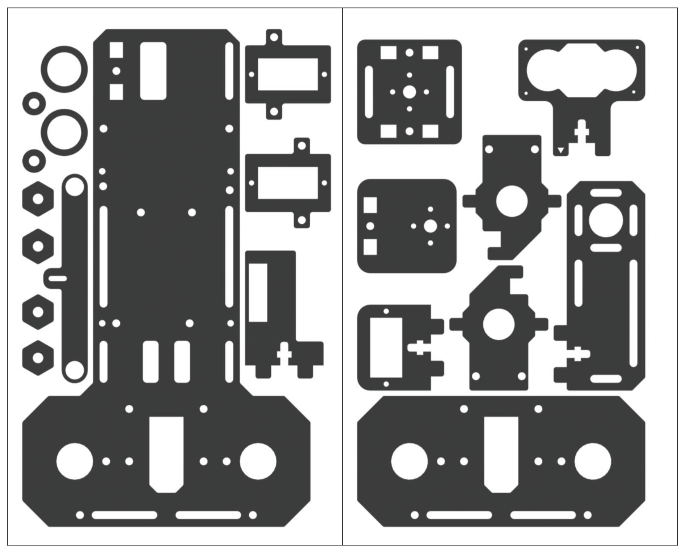
\includegraphics[width=8cm]{img/acrylic_sheets}
\end{figure}

After preparing the main structural components, we mounted the servo motors and sensors onto the respective subassemblies. This required careful placement to ensure proper alignment and functionality.

\begin{figure}[H]
    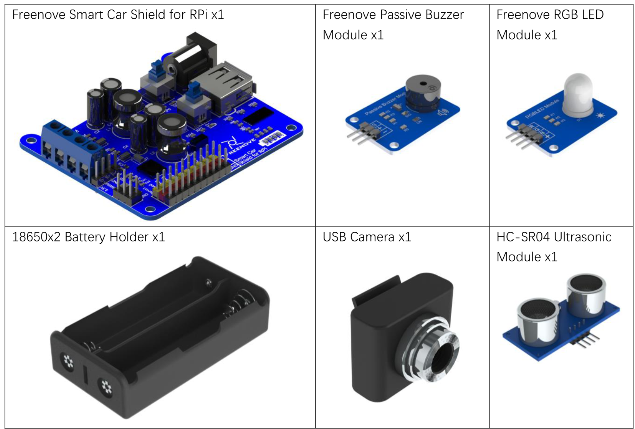
\includegraphics[width=8cm]{img/shield_and_sensors}
\end{figure}

Once all parts were ready, we assembled the full vehicle by attaching the wheels and drive motors to the chassis. At this point, the main mechanical structure of the smart car was completed.

\begin{figure}[H]
    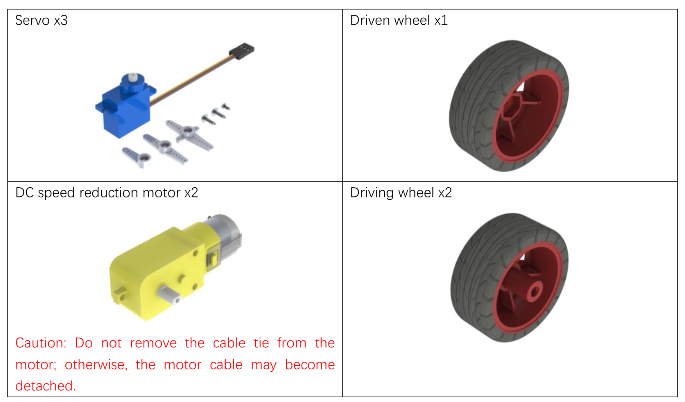
\includegraphics[width=8cm]{img/engine_and_wheels}
\end{figure}

In the final step, we mounted the Raspberry Pi along with the included shield onto the chassis. We inserted the batteries into the holder and connected the motors, sensors, and other components to the shield using jumper cables.

\begin{figure}[H]
    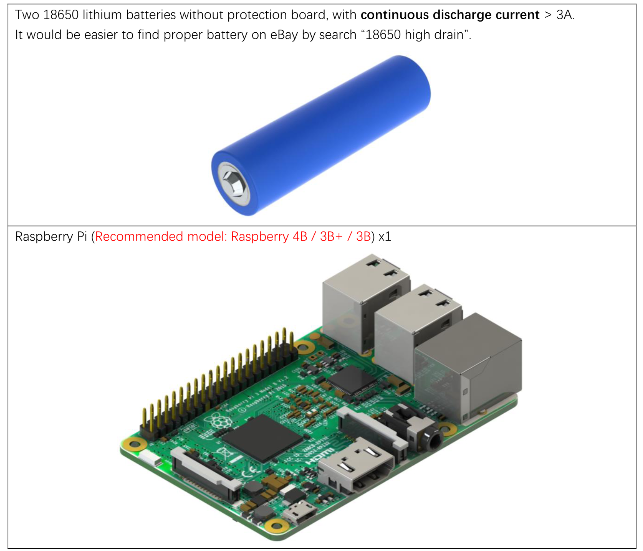
\includegraphics[width=8cm]{img/rpi_and_battery}
\end{figure}

The cables of the individual components were connected to the Raspberry Pi shield according to the pinout shown in the image.

\begin{figure}[H]
    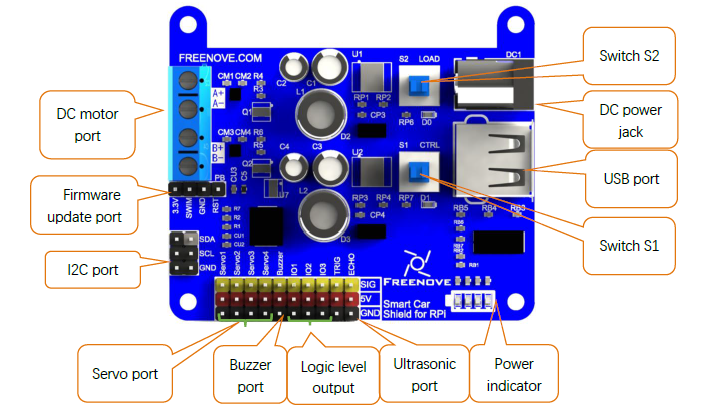
\includegraphics[width=8cm]{img/shield_pinout}
\end{figure}

\subsubsection{Software Setup}

First, we had to flash a micro SD card with an image compatible with the Raspberry Pi. We used the Raspbian Buster Full image and the Raspberry Pi Imager for this task.

Once the image was ready, we powered up the Raspberry Pi and connected it to a temporary display. Then, we connected the Pi to our Wi-Fi hotspot and noted down its IP address to enable remote access via SSH or Remote VNC.

Next, several settings had to be adjusted to allow remote connections:
\begin{itemize}
    \item Enable I2C interface
    \item Enable VNC server
    \item Install XRDP
    \item Adjust screen resolution
\end{itemize}

Finally, we cloned the Git repository for testing purposes:
\begin{verbatim}
git clone http://github.com/Freenove/Freenove_Three-wheeled_Smart_Car_Kit_for_Raspberry_Pi.git
\end{verbatim}

Additionally, we installed several required packages:
\begin{itemize}
    \item i2c-tools
    \item python-smbus
    \item mjpg-streamer
\end{itemize}

After this steps, we were able to connect to the RPi remotely.
\begin{figure}[H]
    
\includegraphics[width=8cm]{img/buster_desktop_background}
\end{figure}


\subsubsection{Testing}
After preparing both the hardware and software, we tested the individual servo motors and the drive motors to check if they were working properly.

For this purpose, we used pre-made test scripts from the cloned Git repository:
\begin{verbatim}
python mDev.py servo
python mDev.py buzzer
python mDev.py motor
python mDev.py RGBLED
\end{verbatim}

Once we confirmed that everything was functioning correctly, we could focus on developing our own software.

\subsection{Software}
%TODO Describe how our software works








